\documentclass[12pt]{article}
%%%%%%%%%%%%%%%%%%%%%%%%%%%%%%%%%%%%%%%%%

\usepackage{amscd}
\usepackage{amsmath}
\usepackage{amssymb}
\usepackage{amsthm}
\usepackage{amsfonts}

\usepackage{subcaption}
\usepackage{hyperref}
\usepackage{paralist}
\usepackage{epsfig}
\usepackage{verbatim}
\usepackage{graphicx}
\usepackage{color}
\usepackage{booktabs}
\usepackage{multirow}
%\usepackage[all,dvips]{xy}


\setlength{\textheight}{8.5in} \setlength{\topmargin}{0.0in}
\setlength{\headheight}{0.0in} \setlength{\headsep}{0.0in}
\setlength{\leftmargin}{0.5in}
\setlength{\oddsidemargin}{0.0in}
%\setlength{\parindent}{1pc}
\setlength{\textwidth}{6.5in}
%\linespread{1.6}

\newtheorem{definition}{Definition}
\newtheorem{problem}{Problem}

\newtheorem{theorem}{Theorem}[section]
\newtheorem{lemma}[theorem]{Lemma}
\newtheorem{note}[theorem]{Note}
\newtheorem{corollary}[theorem]{Corollary}
\newtheorem{prop}[theorem]{Proposition}

\newenvironment{nscenter}
 {\parskip=0pt\par\nopagebreak\centering}
 {\par\noindent\ignorespacesafterend}

%%%%%%%%%%%%%%%%%%%%%%%%%%%%%%%%%%%%%%%%%

\begin{document}
\thispagestyle{empty}

\bigskip
\bigskip

\begin{nscenter}
\textbf{\Large{A Comparison of Classifications in Handwritten Digit Recognition -- Final Report}}
\end{nscenter}

\bigskip

\begin{nscenter}
{Siyang Xue and Tiancheng Liu}
\end{nscenter}

%This is where you would explain, in detail, what you plan to work on. This should be 1 to 3 pages in length. Here is an example of how you would cite your references in the body of your proposal.

\section{Problem Description}
\label{sec:problem}


Digit recognition has been a wide-spread and high-impact pattern recognition task, due to its simplicity: the background and the foreground (digits) are often well-separated, and the classes (categories) are limited to 10 (10 digits). Many researchers have benchmarked different methods on those datasets. Y. LeCun et al.\cite{lecun1998gradient} extracted their Mixed National Institute of Standards and Technology (MNIST) dataset from the National Institute of Standards and Technology (NIST) dataset, and made it normalized and available on their webpage\footnote{\url{http://yann.lecun.com/exdb/mnist/}}; they also provided early works on different classifications configurations in 1995, where linear classifiers, $k$-NN classifiers, and multiple variations of neural networks are investigated; a more complicated and complete comparisons can be found on the same webpage. A more recent work by CL Liu et al.\cite{liu2003handwritten} benchmarked methods of wider range on multiple datasets, on both feature extraction methods and classification methods.

What proposed is to further and more deeply investigate aspects of the digit recognition task. What we care about is how the different options in the classification pipeline affect the performance:
\begin{inparaenum} [\itshape a\upshape)]
\item How different normalization techniques influence the data quality, and how to provide a measurement (or at least, an intuition) on that;
\item how SIFT \cite{lowe2004distinctive}, HOG \cite{dalal2005histograms} and other feature extraction methods perform on feature extraction/generation; 
\item what is the suitable dimension reduction method for the task;
\item how the classifiers and the parameter setting affect the performance of the task.
\end{inparaenum} 

The problem of digit recognition is a simple image classification problem, and the techniques tested on the dataset can be extended to used in other image classification problems. The computer vision community has shown a consistent interest on the digit recognition, not only because the datasets have relatively small size to validate the assumptions, and to test the new techniques, but also because the task alone is a simplified version of optical character recognition (OCR), which is also worth researching. 


\section{Data Description}
\label{sec:data}
The data we used is MNIST dataset\cite{lecun1998gradient}, which is well-known and widely-used for digit recognition. All data are normalized beforehand -- by bounding-box normalization and centering;

Some important information of the datasets is listed as follows:
\begin{itemize}
\item MNIST: Total training set of 60,000 images; test set of 10,000 images; all the digits are normalized to size $20 \times 20$ and put in the middle of a $28 \times 28$ image.
\end{itemize}

In this final stage of our report, we have extended to work on the full set of MNIST dataset, that is, with 60000 digits as training samples, and 10000 digits as testing data. (In the 50\% report we trained and tested on a randomly sampled subset of MNIST, with 600 digits from each subject(0-9) for training, and 100 digits from each subject for testing). 

\begin{figure}[tbp]
	\centering
	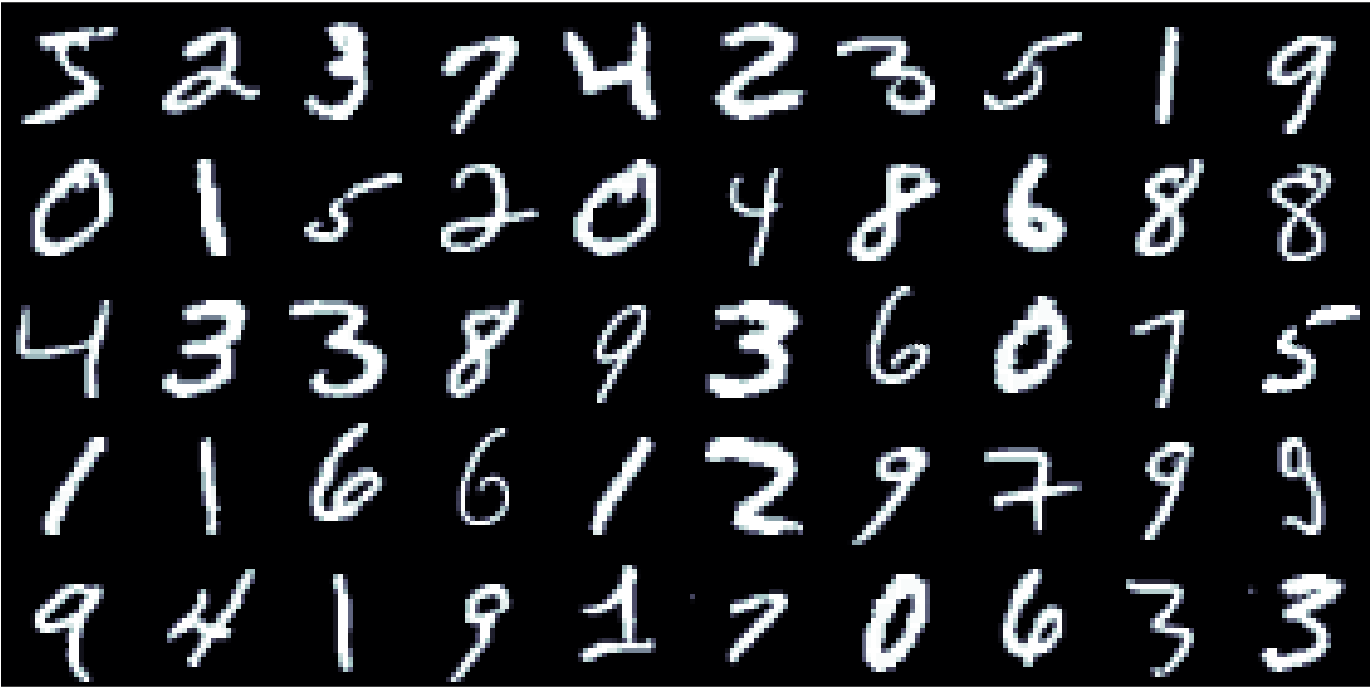
\includegraphics[height = 1.3in]{MNIST}		
	\caption{Digits from MNIST Dataset}
\end{figure}

\section{Methods}
\label{sec:methods}

\subsection{Preprocessing}

The preprocessing step includes 3 sub-steps: normalization, feature extraction/generation, and dimension reduction. 

\subsubsection{Normalization}
The normalization process removes the size variation and brightness variation of the digits. For the MNIST dataset, as suggested by \cite{lecun1998gradient}, we removed the padding area to shrink each image from $28 \times 28$ to $20 \times 20$, which made the matching distance metric more precise and reduced the computational cost of further analysis. All the intensity data are normalized by shifting the mean value to zero, and also normalized by the standard deviation of the pixel values, which removes the brightness variance between different images of digits. The result of the normalization can be seen in Figure \ref{fig:norm}.

\begin{figure}[tbp]
	\centering
	\begin{subfigure}{.45\textwidth}
		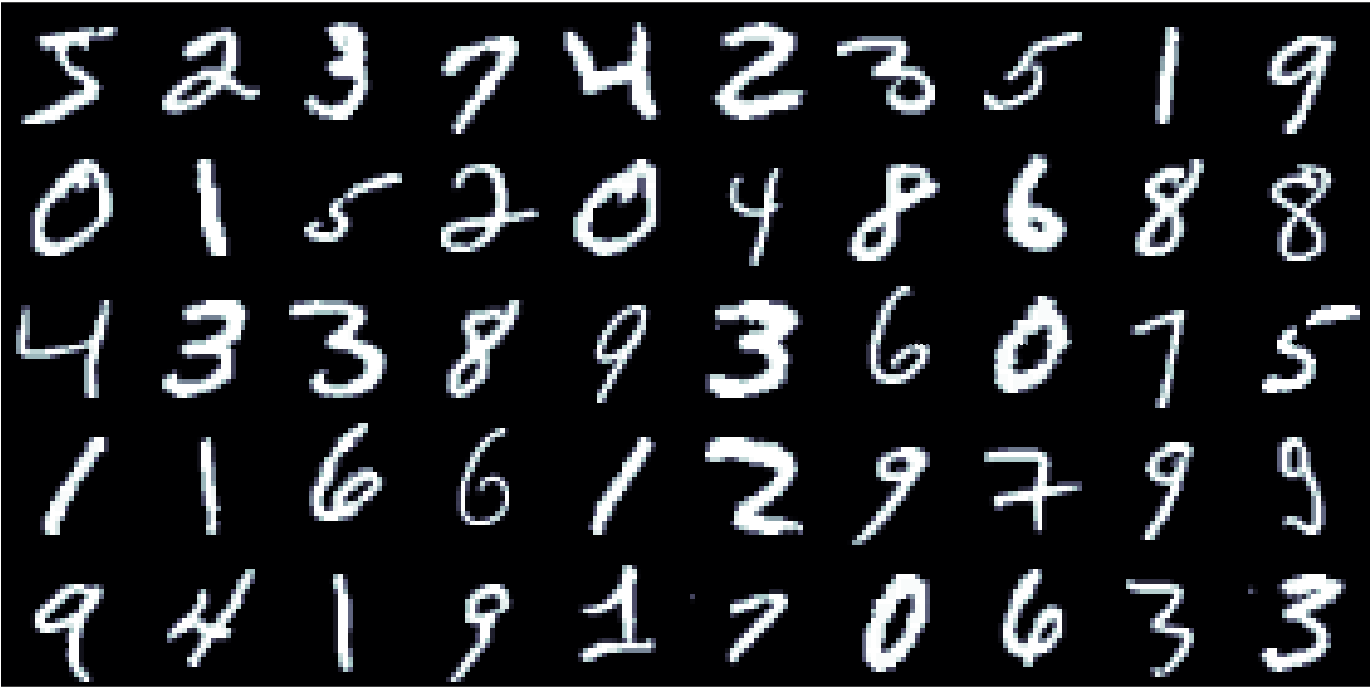
\includegraphics[height = 1.3in]{MNIST}		
		\caption{ }
	\end{subfigure}
	\begin{subfigure}{.45\textwidth}
		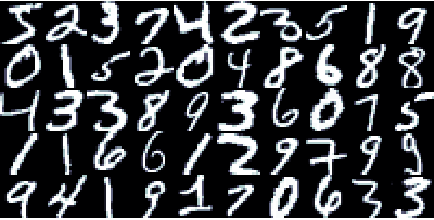
\includegraphics[height = 1.3in]{MNIST_norm}		
		\caption{ }
	\end{subfigure}
	\caption{Normalization of the dataset: (a)~MNIST(original) (b)~MNIST(normalized)}
	\label{fig:norm}
\end{figure}

\subsubsection{Feature Extraction}
Feature extraction/generation methods based on gradient and local invariant feature detectors are investigated. To be specific, in this report, we investigated two common feature extraction strategy in the Computer Vision society: a) HOG features and b) Scale-invariant feature transform (SIFT) features.

\subsubsection*{HOG Features}
 Histograms of Oriented Gradients(HOG)\cite{dalal2005histograms}\cite{felzenszwalb2010object} is a feature extraction method based on detection of local gradient distributions. Not only detection of edge positions, but also intensity normalization is included in this method, making it invariant to the shadows or illumination difference of the sample image. A lot of HOG implementations are proposed, with different parameter and slightly differently designed histogram calculating schemes. In this project, we will focus mainly on a Felzenszwalb et al.\cite{felzenszwalb2010object} version of HOG, for its relatively fewer features in selecting, as we only care about the distinguish from 0 to 9 in handwritten digits recognition, and too many features could result in a input whose dimension is too large for the following classifier.

First, in order to identify the local edge orientation and intensity, the finite difference filter $[-1,0,1]$ and its transpose, are applied to the image to calculate its gradient in 2 directions, the resulting gradient image is then divided into cells of $4\time4$. In each cell, a histogram of the gradient orientation is created by dividing the orientations $\theta$ of the gradient evenly into 9 bins, and each vote has the weight of $r$(i.e. the magnitude of the coordinate pixel). Therefore, for a $ w\times h$ image,  a $w/4 \times h/4 \times 9$ cell feature map $C$ is created. 

Then, in order to achieve an invariance to local gradient bias, for each element of the feature map $C(i,j,:)$, we normalized it together with its 8-neighbor elements and create a $4\times 9$ matrix.
\begin{equation}
\begin{aligned}
HOG(i,j,:,:) =&  \left[\begin{array}{c}
C(i,j,:)./N_{-1,-1}(i,j,:)\\
C(i,j,:)./N_{-1,+1}(i,j,:)\\
C(i,j,:)./N_{+1,+1}(i,j,:)\\
C(i,j,:)./N_{+1,-1}(i,j,:)\end{array}\right]\\
 N_{\delta,\gamma} =&\\
 & (||C(i,j,:)||^2+||C(i+\delta,j,:)||^2+||C(i,j+\gamma,:)||^2+||C(i+\delta,j+\gamma,:)||^2)^{\frac{1}{2}}
\end{aligned}
\end{equation}\cite{felzenszwalb2010object}
Each matrix is then reshaped into a 36 dimensional vector, resulting a overall $ w/4 \times h/4 \times 36$ feature map.

Finally, the now normalized feature map is compressed to 31 features per cell, using PCA projecting the features to 31 most variant dimensions in the $ w/4 \times h/4 $ features of the image. Here, we choose the reduced dimension to 31 according to the singular value decomposition result, in which the last 5 singular values approximate to 0. This step is different from the later dimension-reduction step of all the images in the training set in that it calculates the principal components within the same image and is aimed at eliminating the specific minor noises of a particular image.
\begin{figure}[h]
\centering
	\begin{subfigure}{.85\textwidth}
		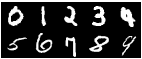
\includegraphics[height = 2.1in]{image.png}		
		\caption{ }
	\end{subfigure}
	\begin{subfigure}{.85\textwidth}
		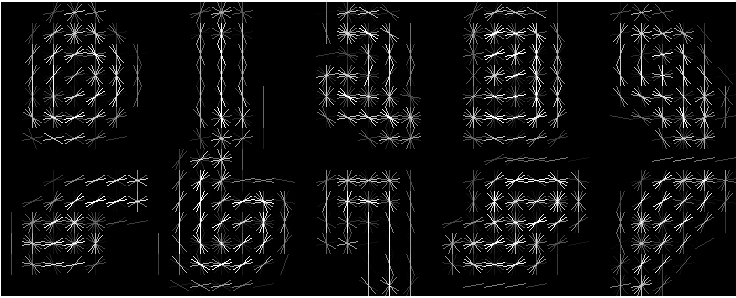
\includegraphics[height = 2in]{hog.png}	
		\caption{ }
	\end{subfigure}
	\caption{ (a)handwritten digits 0-9 from MNIST (b)HOG features of handwritten digits 0-9}
	\label{fig:hog}
	\end{figure}

The original images, and the HOG features of digits from 0 to 9 are shown in Figure \ref{fig:hog}(a) and Figure \ref{fig:hog}(b), respectively. As shown in the figures, the HOG features well describe the outlines of the digits. A digit written with a thinner line( such as the '9' in Figure 1) does not make much difference in the HOG feature description with digits written with thicker strokes, making the features resistant to the irrelevant factors.
\subsubsection*{SIFT Features}
 
Scale-invariant feature transform is a popular feature extraction technique introduced by David Lowe in his 2004 paper \cite{lowe2004distinctive}. The process consists of typically three steps: a) Detection of scale-space extrema, where image pyramid is generated using a set of different-scaled Gaussian kernels, and the extrema is detected in a spatial-hierarchical neighborhood; b) Accurate keypoint localization, where the extrema of low contrast and extrema near the image boundary are discarded; c) Orientation assignment, where each keypoint is assigned several orientations according to its spatial neighbors.

The SIFT features are often applied in object detection, face recognition, and other related tasks \cite{yilmaz2006object, dalal2005histograms}, due to its robustness against image scaling, image rotation, and certain kinds of noise. In these applications, the SIFT features (keypoints) are extracted, and oftentimes, it is followed by extracting the HOG features of the spatial neighborhood of the keypoints, to generate a feature descriptor \cite{lowe2004distinctive}.

However, this feature extraction strategy is ineffective for the MNIST dataset. In the experiment, we found all the images have only a few feature points to be extracted ($\leq 4$), which is insufficient to describe the image (see Figure \ref{fig:SIFT}); some image even failed on SIFT, that means it have no SIFT feature to extract. Furthermore, it may not be a desirable choice for digits dataset, where we have 6 and 9 with the same topology, and the rotation invariant property of SIFT would made it impossible to distinguish the above 2 digits. Therefore, in this report, we do not use SIFT as a feature extraction technique, and only HOG is used to generate feature descriptors.

\begin{figure}[tbp]
	\centering
	\begin{subfigure}{.45\textwidth}
		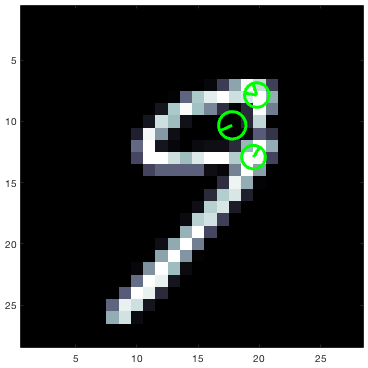
\includegraphics[height = 2.5in]{SIFT}		
		\caption{ }
	\end{subfigure}
	\begin{subfigure}{.45\textwidth}
		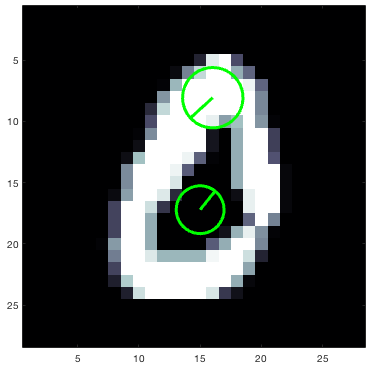
\includegraphics[height = 2.5in]{SIFT_2}		
		\caption{ }
	\end{subfigure}
	\caption{Handwritten digits with their SIFT features: (a)~A handwritten 9 (b)~ A handwritten 0}
	\label{fig:SIFT}
\end{figure}


However, for further study, if we are to investigate faces, SIFT would be a good choice for extracting the keypoints in a more complex context, and the the invariant properties of the SIFT would help the recognition.
 
\subsubsection{Dimension Reductions}
 
The dimension reduction methods used in this report can be categorized into 2 groups: linear and nonlinear. For linear method, we apply the conventional PCA; both kernel method (Kernel-PCA) and manifold learning method (LLE) are investigated as nonlinear methods. Experiments are conducted to compare the effectiveness and efficiency of the methods.

\subsection{Classification}
Three different classification methods are used in this report. $k$-NN\cite{altman1992introduction} classifier is used for investigating the dimension reduction methods; several experimental comparisons based on $k$-NN classifiers are conducted to highlight the difference of the performance, and to give a clue about what are the desirable preprocessing methods for digit recognition tasks. The SVM classifiers are reported as desirable classifiers of the task because of its high-accuracy, flexibility in its kernel choices, and also low-computational complexity \cite{soltanzadeh2004recognition, bottou1994comparison, liu2003handwritten}; on the other hand, the SVM classifiers are sensitive to kernel choice, and in terms of feature transformation, the ``kernel tricks'' that we used in the dimension reduction methods are already transformed the feature space according to the kernels, and it might not be desirable to use the kernels a second time. In early literature, neural networks are proposed to solve the problem of handwritten digits recognition, and the accuracies are comparable to SVM classifiers \cite{le1990handwritten, lecun1995comparison} despite its high computational cost in training process. In recent years, the trend of deep learning brings back convolutional neural network (CNN), and the state-of-art results are obtained by CNNs \cite{krizhevsky2012imagenet,cirecsan2011convolutional, ciresan2012multi}.

\subsubsection{$k$-NN Classifier}

The $k$-NN\cite{altman1992introduction} Classifier we used in the project is based on euclidean distance ($l2$-norm), such that for any two feature vectors $\mathbf{x}$ and $\mathbf{y}$, the distance between are defined as
\begin{equation}
	d({\bf x}, {\bf y}) = \|{\bf x} - {\bf y}\|_2^2
\end{equation}

The performance of the classifications are measure by the overall accuracy (OA), that is, the ratio of corrected labeled feature vectors (digits) in all feature vectors. The pipeline that we used with $k$-NN classifier can be seen in Figure \ref{fig:pipeline-knn}.

\begin{figure}[tbp]
	\centering
	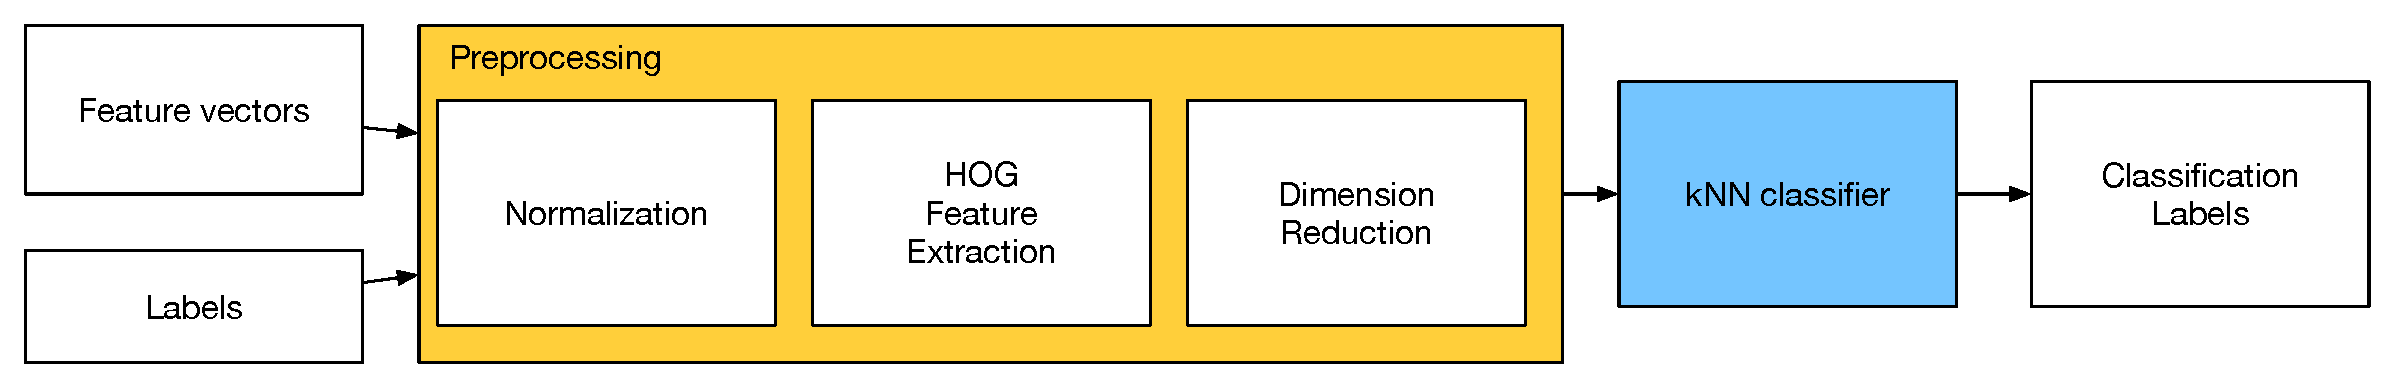
\includegraphics[width =\textwidth]{pipeline-knn}		
	\caption{The classification pipeline with $k$NN classifier}
	\label{fig:pipeline-knn}
\end{figure}

In this report, in order to highlight the effect of the preprocessing steps, we have different settings of parameters, the parameter settings are as follows:
\begin{itemize}
	\item With/without normalization
	\item With/without HOG feature extraction
	\item Dimension Reduction: \{None, PCA with kernel: {Linear, Polynomial, Gaussian}, LLE\}
\end{itemize}
Thus we have a total of $2 \times 2 \times 4 = 16$ different classification instances.

\subsubsection{SVM Classifier}

Support vector machine (SVM)\cite{le1990handwritten, lecun1995comparison} finds the hyperplane that best seperates the two classes in the high-dimensional space. According to representer theorem, the solution of the optimization problem can be expressed in another space by a linear combination of inner products defined in that space. That is, the ``kernel trick'' allows us to tranform the feature space into another Rreproducing Kernel Hilbert Space (RKHS), and hence find the nonlinear boundary between the classes in the original feature space. The performances of the SVM classifiers are sensetive to the kernel types and parameters.

In this report, we investigate 3 different kernel of SVM classifiers in this report: linear kernel, polynomial kernel, and radial basis function (rbf) kernel. For the polynomial kernel, we tried different values of degree $d$, where $d \in \{2,3,5,7\}$; for rbf kernel, we tried the standard deviation $\sigma \in \{3, 4, 5, 7\}$. As mentioned before, the SVM classifiers transformed the features by theirselves according to the kernels, and thus the classification pipeline with SVM classifier is shown in Figure \ref{fig:pipeline-svm}.

\begin{figure}[tbp]
	\centering
	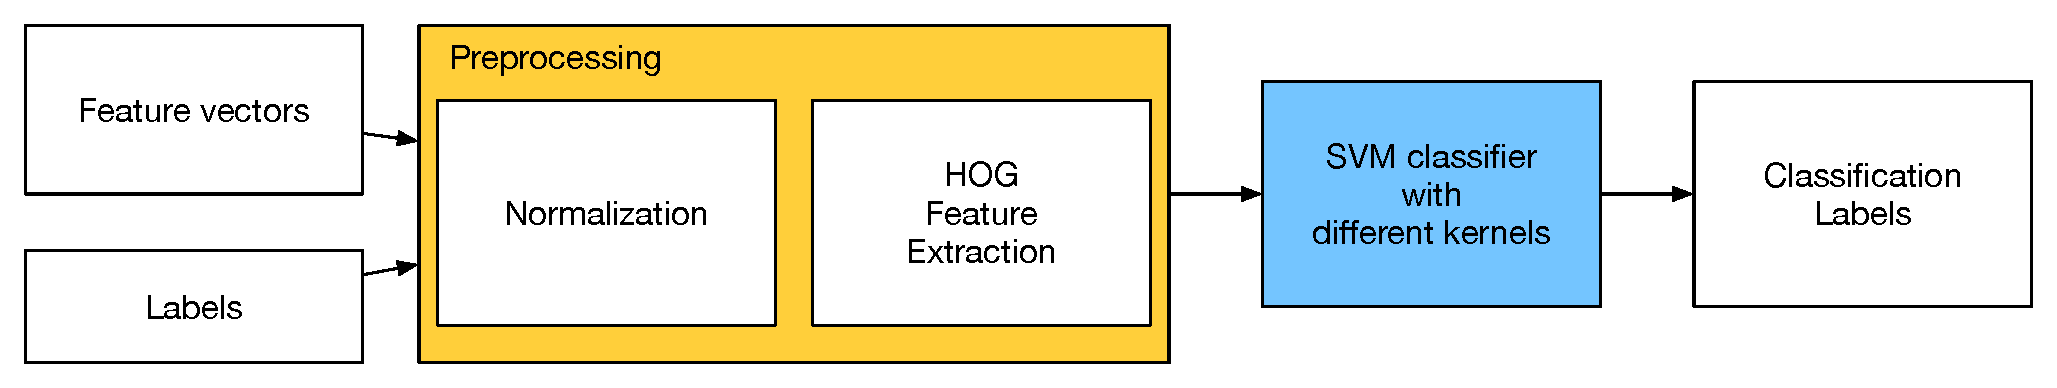
\includegraphics[width =\textwidth]{pipeline-svm}		
	\caption{The classification pipeline with SVM classifier}
	\label{fig:pipeline-svm}
\end{figure}
 
\subsubsection{CNN Classifier}
Convolutional Neural Networks(CNN)\cite{krizhevsky2012imagenet}, which intuitively pulls its layers within the receptive fields of each units, just like extracting features from lower to higher levels. This hierarchy enables CNN to capture the overall topological properties of the objects more easily and improves the performance of recognition incredibly\cite{lecun1998gradient}.
The organization of CNN is built in the following steps: 

1. For each layer of the network, let the input image I be of $n \times n$ pixels, and let the receptive fieild of each pixels be a square of $r\times r$ (here, R is a small odd number), let $K_i$ represents the $r\times r$ kernels;

2. Calculate the convolution of I and $K_i$($i = 1,2...,m$), resulting m images of $(n-r+1) \times (n-r+1)$;

3. Down-sample the images with stripe s, the output of this layer is built up with the resulting m $(n-r+1)/s \times (n-r+1)/s$ images;
\subsubsection{Preprocessing}

In order to fit the input image in the overall architecture of the convolutional networks, each $28\times 28$ input image is put in an all-zero matrix of $32\times 32$(details in the following section).

\subsubsection{Overall Architecture}

As shown in Figure \ref{fig:arch}, our neural network is built up of 3 layers of convolutional networks and 2 fully-connected neural networks. The initial input of the network is a $32\times 32$ matrix, and with 6 convolutional $5\times 5$ kernels in layer 1, and down-sampling stripe 2, the resulting output are 6 $14\times 14$ images. Similarly, the number of $5\times 5$ kernel for layer 2 is 16 and the down-sampling rate is 2, resulting in 16 $5\times 5$ images. Finally, with no down sampling and 120 $5\times 5$, the output of layer 3 is exactly 120 $1\times 1$ units.

\begin{figure}[tbp]
	\centering
	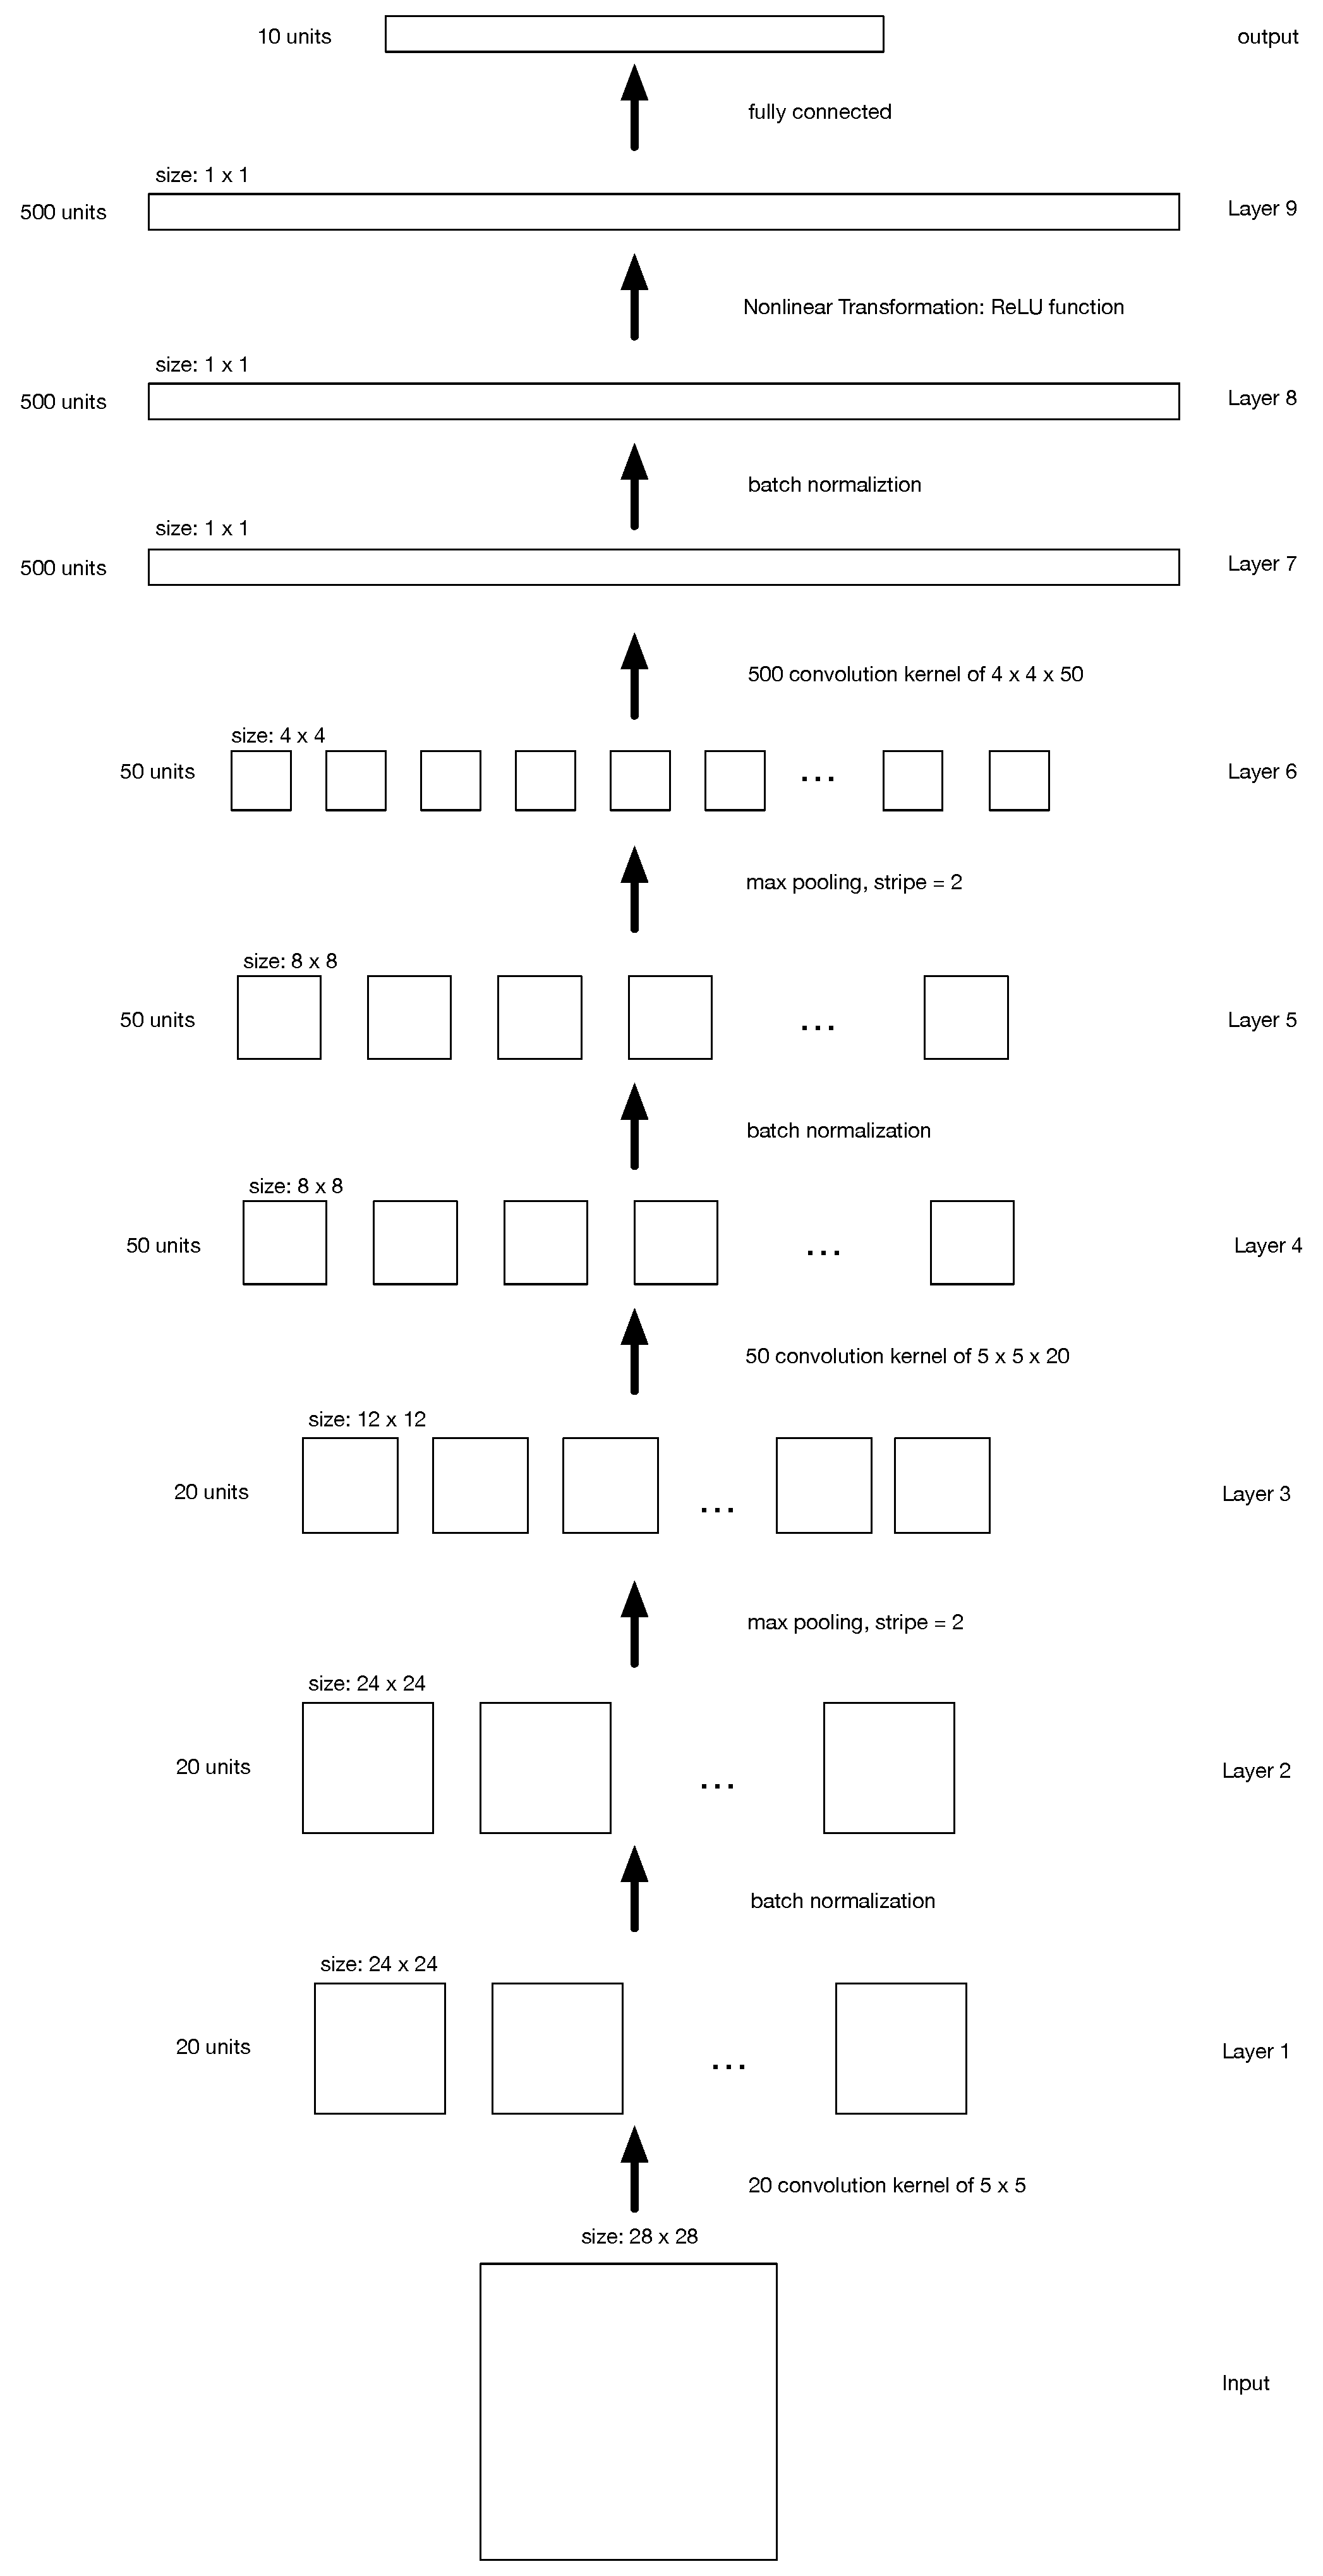
\includegraphics[width =0.65\textwidth]{cnn_arch}		
	\caption{The architecture of CNN}
	\label{fig:arch}
\end{figure}

\begin{figure}[tbp]
	\centering
	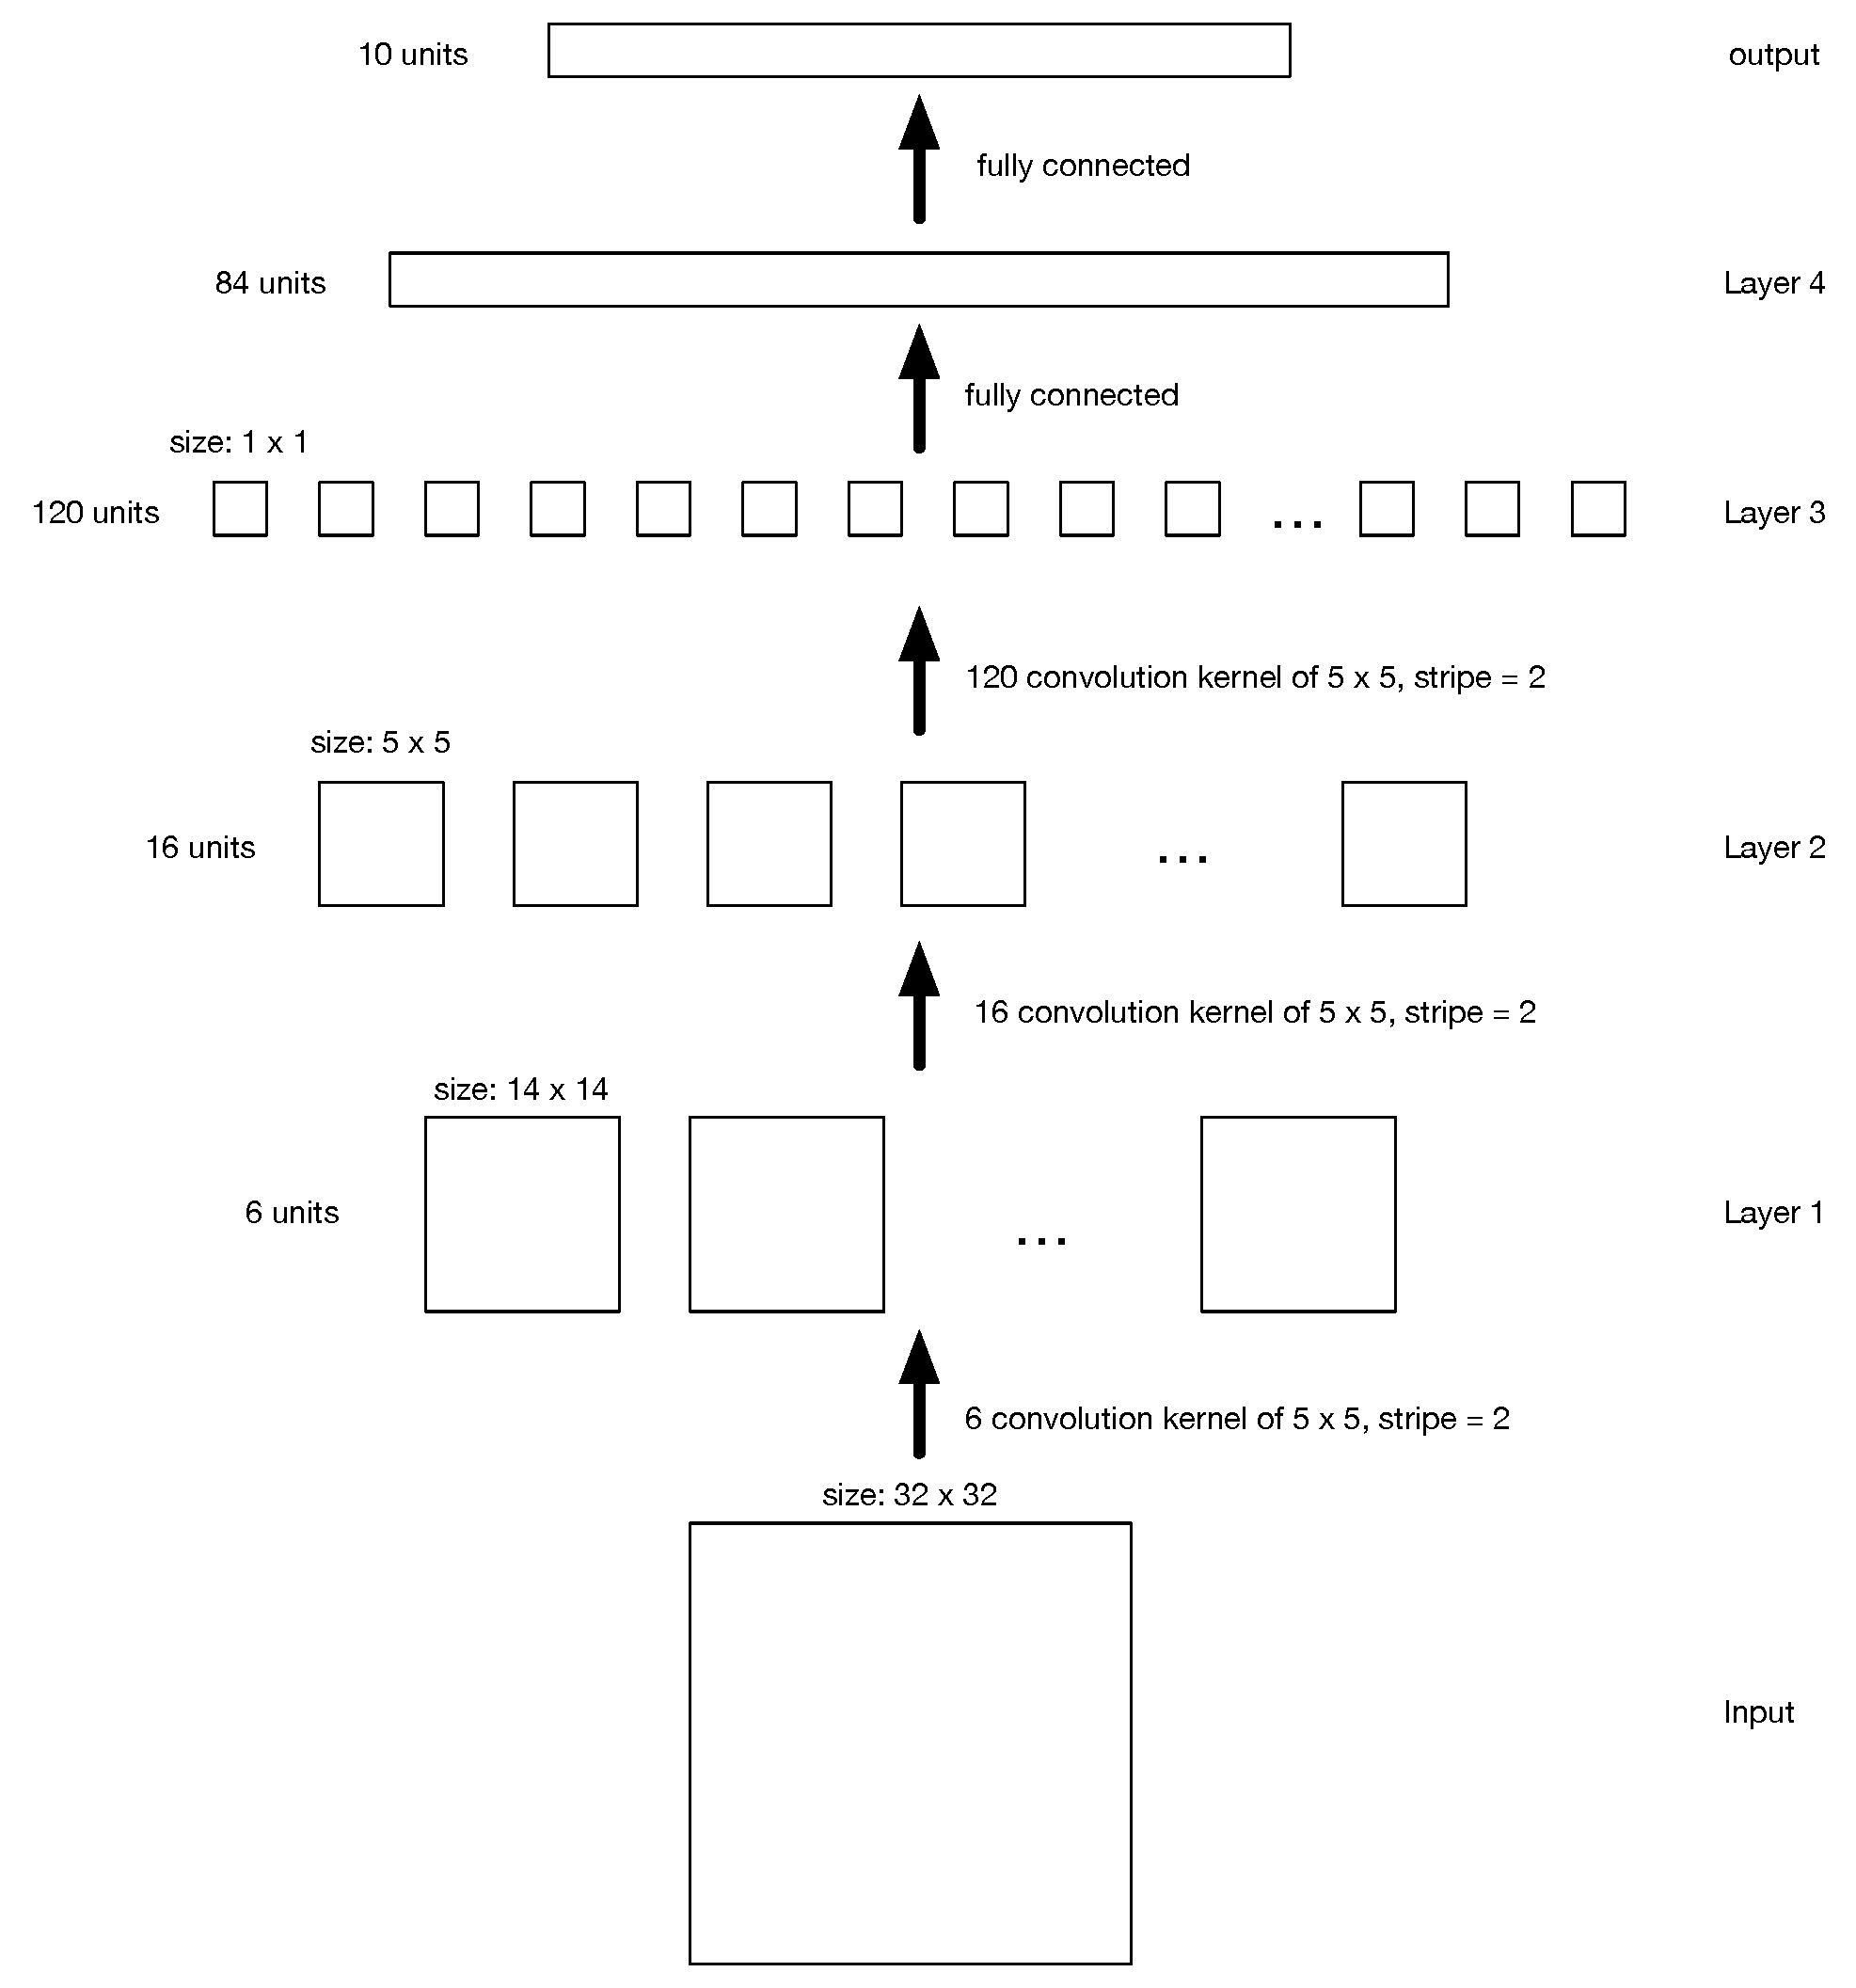
\includegraphics[width = 0.65\textwidth]{cnn}		
	\caption{The architecture of CNN}
	\label{fig:arch}
\end{figure}

The following 2 fully connected layers acts as hierarchical classifiers: 84 sub-features are first selected from the 120 features, and are then classified into 10 classes of digit 0 to 9.

We choose the kernel size  $5\times 5$ as this size would best characterize the local features, without too much overlapping but still have padding between the neighbor output, and the number of kernels are chosen roughly empirically, for fewer kernel features will affect the performance while  an increase in the number of features leads to no obvious improvement. 


\subsubsection{Training}

The training of the CNN follows the back-propagation learning scheme\cite{lecun1989backpropagation}, which fits the input with the standard output by minimizing its training error.
In our project, there are altogether $5\times 5\times(6+16+120)+121\times84+85\times10 \approx 12000$ parameters, which means the training process is extremely time-consuming. 
(We reference the original training parameter to the work of Patrice Y. Simard \cite{simard2003best})


\section{Results}
\label{sec:res}

\subsection{$k$-NN classifier}
In this section, we discuss the differences of the performances of the classifier with input types: features without selection, HOG features selected with raw data, and further HOG features selected with normalized data over the several dimensional reduction methods. Running time and classification accuracy are both included in the measurement of the performance. The results can be seen in Figure \ref{fig:knn} and Table \ref{tab:knn}.

\begin{figure}[tbp]
	\centering
	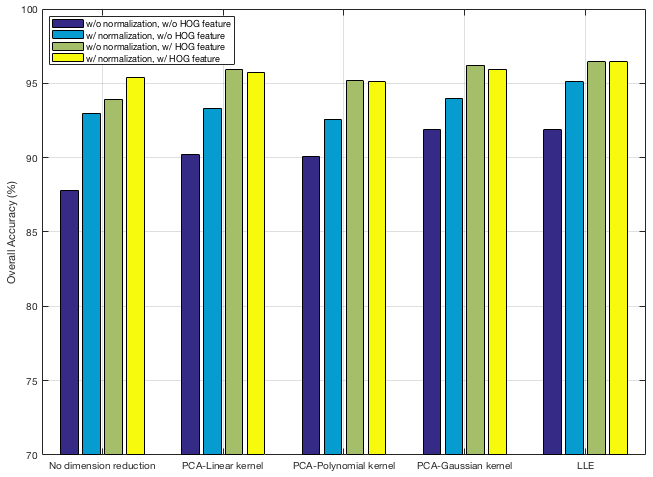
\includegraphics[width =\textwidth]{knn}		
	\caption{The result of digit recognition of classification pipeline with $k$NN classifier}
	\label{fig:knn}
\end{figure}

\begin{table}[]
\centering
\caption{Accuracy and running time of classification pipeline with $k$-NN classifier on average}
\label{tab:knn}
\resizebox{0.95\textwidth}{!}
{
\begin{tabular}{@{}cccccccc@{}}
\toprule
\multirow{3}{*}{}                                                                                   & \multirow{3}{*}{Normalization} & \multirow{2}{*}{\begin{tabular}[c]{@{}c@{}}HOG\\ Feature\end{tabular}} & \multirow{3}{*}{\begin{tabular}[c]{@{}c@{}}No \\ Dimension\\ Reduction\end{tabular}} & \multicolumn{3}{c}{Kernel PCA} & \multirow{3}{*}{\begin{tabular}[c]{@{}c@{}}Locally Linear\\ Embedding\\ (LLE)\end{tabular}} \\ \cmidrule(lr){5-7}
                                                                                                    &                                &                                                                        &                                                                                      & \multirow{2}{*}{Linear} & \multirow{2}{*}{Polynomial} & \multirow{2}{*}{Gaussian} &                                                                                             \\
																									&                                &                                                                        &                                                                                      &  &  & &                                                                                             \\ \midrule
\multirow{4}{*}{\begin{tabular}[c]{@{}c@{}}Overall\\ Classification\\ Accuracy\\ (\%)\end{tabular}} & w/o                            & w/o                                                                    & 87.80                                                                                & 90.20  & 90.10      & 91.90    & 91.90                                                                                       \\
                                                                                                    & w/                             & w/o                                                                    & 93.00                                                                                & 93.30  & 92.60      & 94.00    & 95.10                                                                                       \\
                                                                                                    & w/o                            & w/                                                                     & 93.90                                                                                & 95.50  & 95.20      & 96.20    & 96.50                                                                                       \\
                                                                                                    & w/                             & w/                                                                     & 95.40                                                                                & 95.70  & 95.10      & 95.90    & 96.50                                                                                       \\ \midrule
\multirow{4}{*}{\begin{tabular}[c]{@{}c@{}}Running\\ Time\\ (s)\end{tabular}}                       & w/o                            & w/o                                                                    & 2.50                                                                                 & 5.72   & 76.68      & 80.20    & 38.95                                                                                       \\
                                                                                                    & w/                             & w/o                                                                    & 0.50                                                                                 & 0.61   & 73.50      & 76.91    & 18.71                                                                                       \\
                                                                                                    & w/o                            & w/                                                                     & 14.70                                                                                & 17.01  & 99.61      & 107.39   & 101.39                                                                                      \\
                                                                                                    & w/                             & w/                                                                     & 7.24                                                                                 & 7.98   & 92.52      & 101.76   & 45.01                                                                                       \\ \bottomrule
\end{tabular}
}
\end{table}

\subsubsection{Comparison on Normalization}
As can be seen in Table \ref{tab:knn}, both the HOG feature extraction and normalization process raise the performance of classification; however, the normalization process with HOG feature extraction does not always outperform the pipeline with HOG features alone regrading the overall accuracy, but at the same time, the running time of the former are always less than the latter, which demonstrates that the computational complexity is reduced. 

\subsubsection{Comparison on Feature Selection}
As can be seen in Table \ref{tab:knn}, basically a increase of accuracy of 4\% to 7\% is achieved by selecting HOG features. Better edge detection and shadow invariant property of the HOG features might contribute to this increase. The increase is especially large in the case of no dimension reduction ( 7.6\% ) as the classification performance is more dependent to the feature quality with no further dimension reduction step.
The running time is longer with feature selection, as the original dimension of the data is 784, and the selected feature dimension here is 775, so there is no much decrease in the dimension reduction process, and the increase in computational complexity comes from the HOG feature detection step. This increase, however, is minor (less then 10 percent) compared to the accuracy improvement.

\subsubsection{Comparison on Dimension Reduction Methods}
The dimension reduction methods we used for this project are kernel-PCA and Locally Linear Embedding (LLE). While we include PCA with linear kernel in the comparison, the comparison include 3 different scenes, while the last scene can also be divided into 2 groups:
\begin{itemize}
	\item No dimension reduction
	\item dimension reduction with linear assumption: PCA with linear kernel
	\item dimension reduction with nonlinear assumption:
	\begin{itemize}
		\item kernel-based dimension reduction: PCA with polynomial kernel and PCA with gaussian kernel
		\item manifold-based dimension reduction: LLE
	\end{itemize}
\end{itemize}

As we can see in Figure \ref{fig:knn} and Table \ref{tab:knn}, we can seen that LLE is the desirable dimension reduction method in the task, because it reached a high accuracy, and also of relative low computational cost compared to kernel-based nonlinear dimension reduction methods.

\subsection{SVM classifier}

SVM classifier is also investigated in this report, we apply the SVM classifier on the HOG features. The reason that we do not use the SVM on the dimension reduction is that the kernel of SVM itself already transformed the feature space.

The overall accuracy of the linear-kernel based SVM is 96.80\%, which is comparable to the best result before with the $k$-NN classifier.


Consider the polynomial kernel, the overall accuracy drops a little bit when the degree of polynomial goes higher, as we can seen in Figure \ref{fig:svm-poly}. This phenomenon suggests that the overfitting is more likely to occur when the degree goes higher, and also, the accuracy is not necessarily related to the complexity of the kernel that are using. The best result of polynomial-kernel based SVM is 97.60\%.
\begin{figure}[tbp]
	\centering
	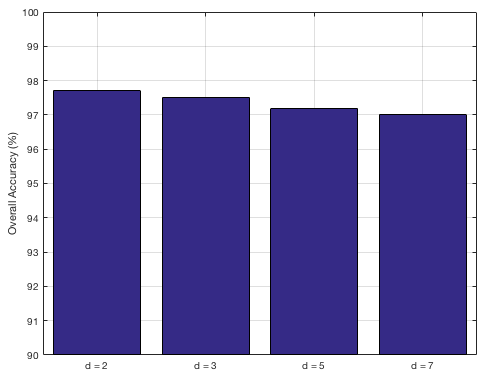
\includegraphics[width = 0.6\textwidth]{svm}		
	\caption{The classification accuracy of SVM with polynomial kernels under different degrees}
	\label{fig:svm-poly}
\end{figure}

With the rbf kernel, the accuracy also change with different parameter $\sigma$, as can seen in Figure \ref{fig:svm-rbf}. With $\sigma = 4$, we reached an overall accuracy of $97.8\%$, which is the best among all the classification results of SVM classifiers.

\begin{figure}[tbp]
	\centering
	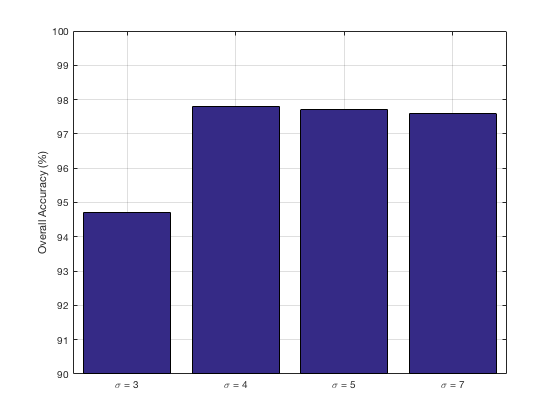
\includegraphics[width = 0.6\textwidth]{svm-rbf}		
	\caption{The classification accuracy of SVM with rbf kernels under different $\sigma$}
	\label{fig:svm-rbf}
\end{figure}


\subsection{CNN classifier}

The overall accuracy of CNN classifier is 93\%, which is below the overall accuracy of both $k$-NN classifiers with dimension reduction and SVM classifiers. However, this is expected because the CNN requires a huge size of training samples to determine the weights, and we are planning to investigate on the elastic and affine distortions that are introduced in the literature \cite{cirecsan2011convolutional, ciresan2012multi} to enlarge the dataset in the future.

\section{Conclusion}
\begin{itemize}
	\item Preprocessing:
	\begin{itemize}
		\item HOG feature: the HOG feature utilized the higher-order information of the feature vector (gradients), which added discrimination between the classes. However, the HOG feature has a higher dimensionality than the original features, thus may increase the computational complexity of the classification step.
		\item SIFT feature: the SIFT descriptor is based on topology, and has a rotation invariant property, thus may not be suitable for digit recognition. Moreover, the number of descriptors found in the each image (feature vector) may not be the same, which complicated the further classification task, where the dimensionality of the feature varies.
	\end{itemize}
	\item Classifiers:
	\begin{itemize}
		\item Dimension reduction with $k$-NN: the dimension reduction methods explicitly transform the feature space. This method has a simple algorithm structure, but has a relatively high error rate. In the experimental comparison of the dimension reduction methods, Locally Linear Embedding (LLE) has the highest accuracy and relatively low computational complexity, thus is suitable for the digit recognition task.
		\item Support Vector Machine (SVM): SVM has a fast training process and a relatively high accuracy. However, this classifier is sensitive to kernel choice, thus need prior knowledge of the dataset.
		\item Convolutional Neural Network (CNN): the CNN renders the highest accuracy both in the literature and in our report. In the literature, the best single CNN has reached a 99.65\% accuracy. In our experiments, the accuracy is 99.18\%. Another strength of CNN is that is requires less preprocessing, where the convolution layers can be seen as feature extraction steps. CNN is a model-based method, thus once the coefficients are determined by the training process, the testing process will be a lot more time-efficient. However, the CNN tend to overfit the data, thus need a large training set, and the training process is time-consuming.
	\end{itemize}
\end{itemize}

\bibliographystyle{plain}
\bibliography{references}


\newpage
\begin{nscenter}
\Large{Tiancheng's contribution}
\end{nscenter}
\begin{itemize}
\item Investigate the literature of SVM classifiers on digit recognition
\item Write the functions and scripts for SVM classifier
\item Rewrite the scripts for normalization methods to make the feature vectors zero-mean and standard deviation of 1.
\end{itemize}

\newpage
\begin{nscenter}
\Large{Siyang's contribution}
\end{nscenter}
\begin{itemize}
\item Investigated the HOG, and discussed how it improved the performance of classification by detecting edges more accurately
\item Running the experimental comparison between the feature selected and none feature selected classification.
\item Fixed the kernel-PCA code
\end{itemize}



%%%%%%%%%%%%%%%%%%%%%%%%%%%%%%%%%%%%%%%%%






\end{document} 
